%___________________________________________
%*************************************************************
% Results
%___________________________________________
%^^^^^^^^^^^^^^^^^^^^^^^^^^^^^^^^^^^^^^^^^^^^^^^^^^^

\section{Results}

%-----------------------------------------------------------------------
% Learning Results
%-----------------------------------------------------------------------

\subsection{Learning Data}

\afterpage{
\begin{landscape}
 \begin{figure}
  \centering
  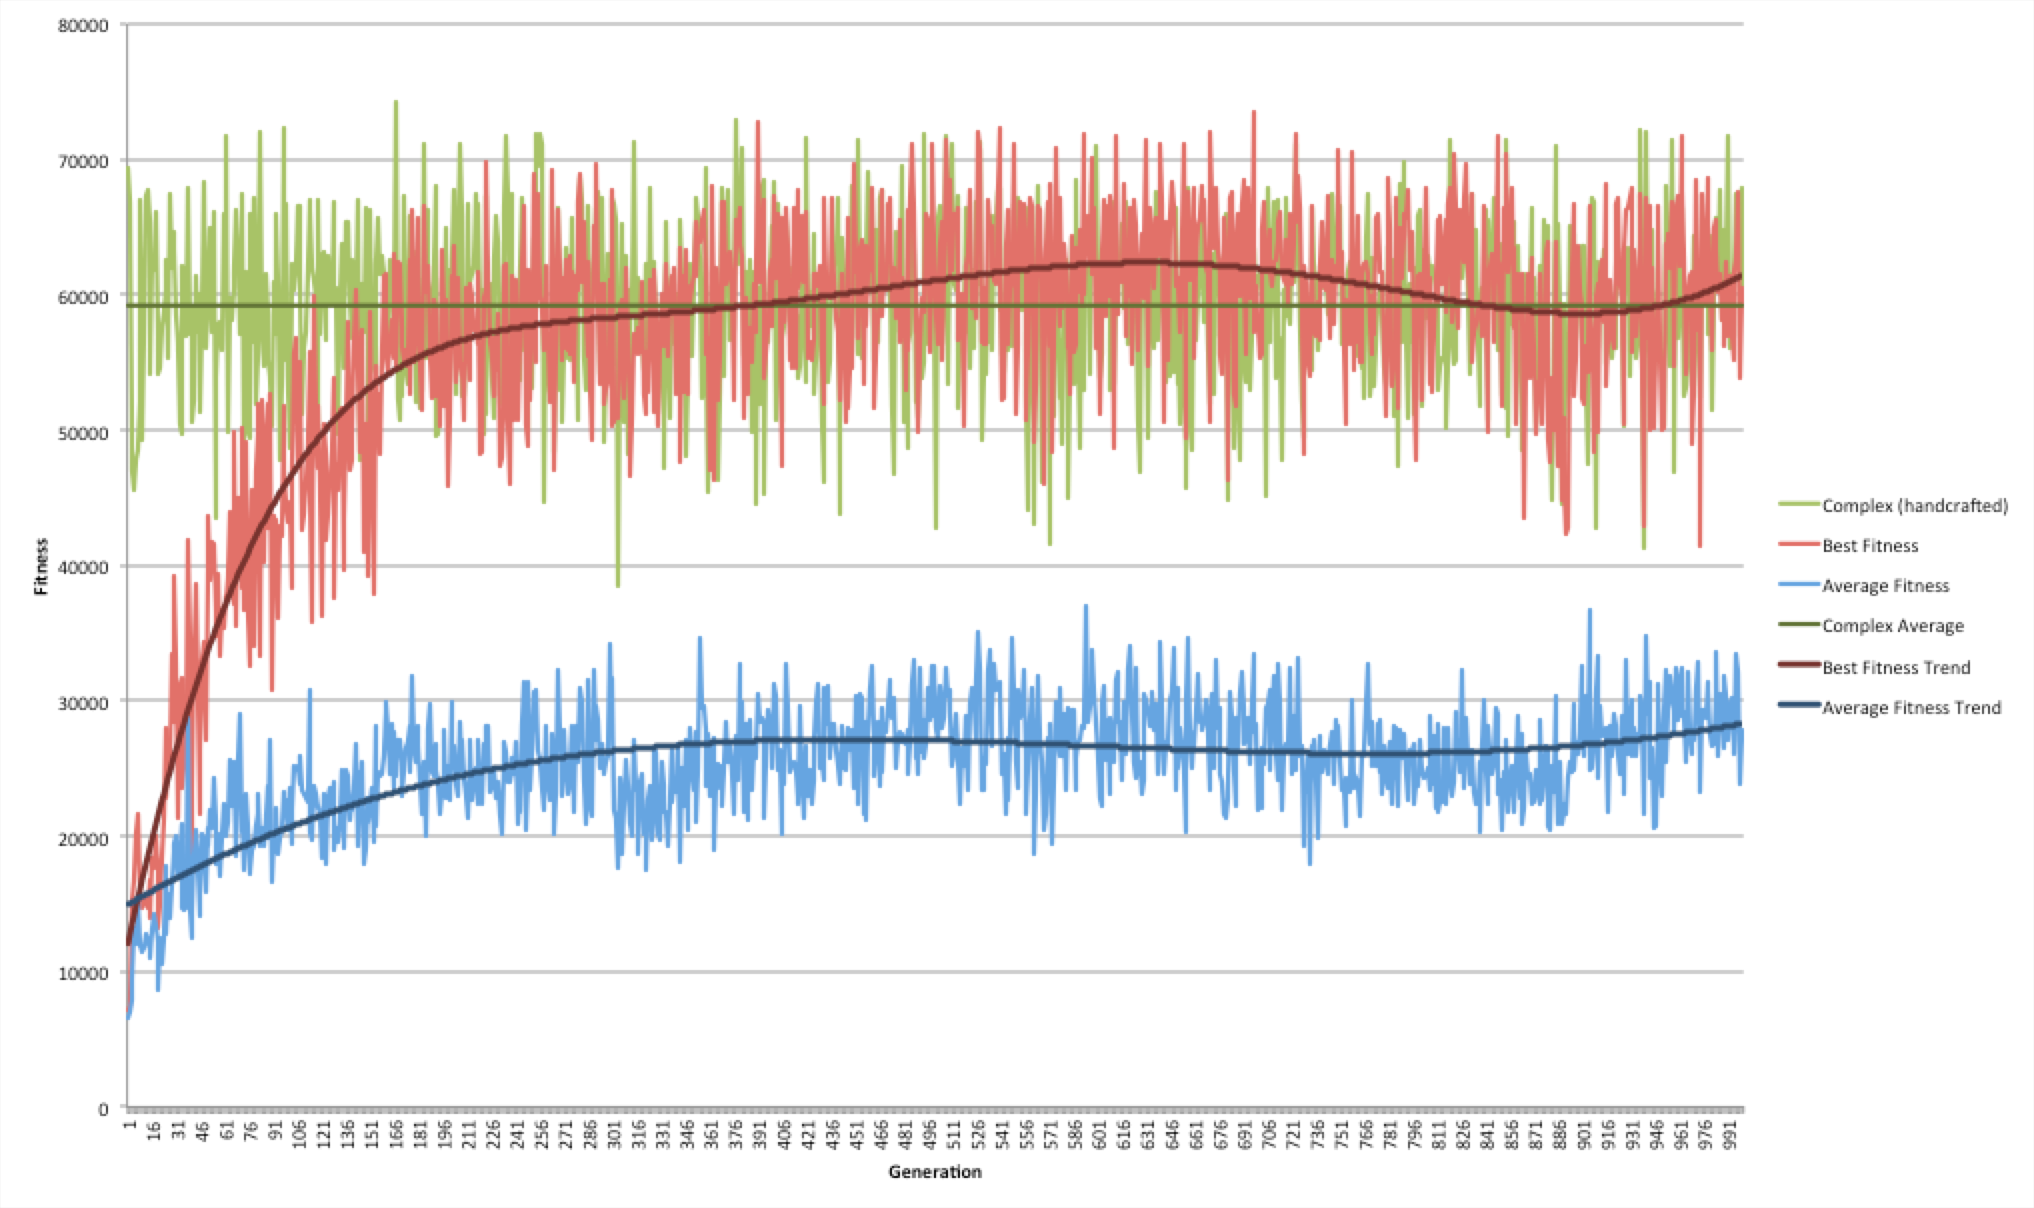
\includegraphics[scale=0.6]{LearnGraph.png}
  \caption{Graph charting the best and average fitness over the final learning run. Handcrafted \textbf{complex} agent fitness also included.}
  \label{fig:learngraph}
 \end{figure}
\end{landscape}
}

\begin{itemize}
\item Statistics output of learning module collated and organised.
\item Figure \ref{fig:learngraph} shows the data in graphical form. It includes the best and average fitness of each generation, with polynomial trend line.
\item Fitness of the handcrafted agent (on playing same levels) also included for comparison.
\item Agents evolved during this run are analysed in more detail in Section \ref{subsec:evallearnt}.
\end{itemize}

\subsubsection{Improvement over Time}

\begin{itemize}
\item Graph shows improvement in both average and best fitness.
\item During early generation improvement is rapid, but slows considerably after 200 generations.
\item Mainly due to agents saturating the evaluation task; 70,000 is a very high score, marking the completion of all levels. Anything over 60,000 is very capable agent (in terms of evaluation task).
\item We also see form the trend line that the best fitness is often better than the handcrafted complex agents fitness.
\end{itemize}

\clearpage

\subsubsection{Generation Variance}

\begin{figure}[t]
	\centering
	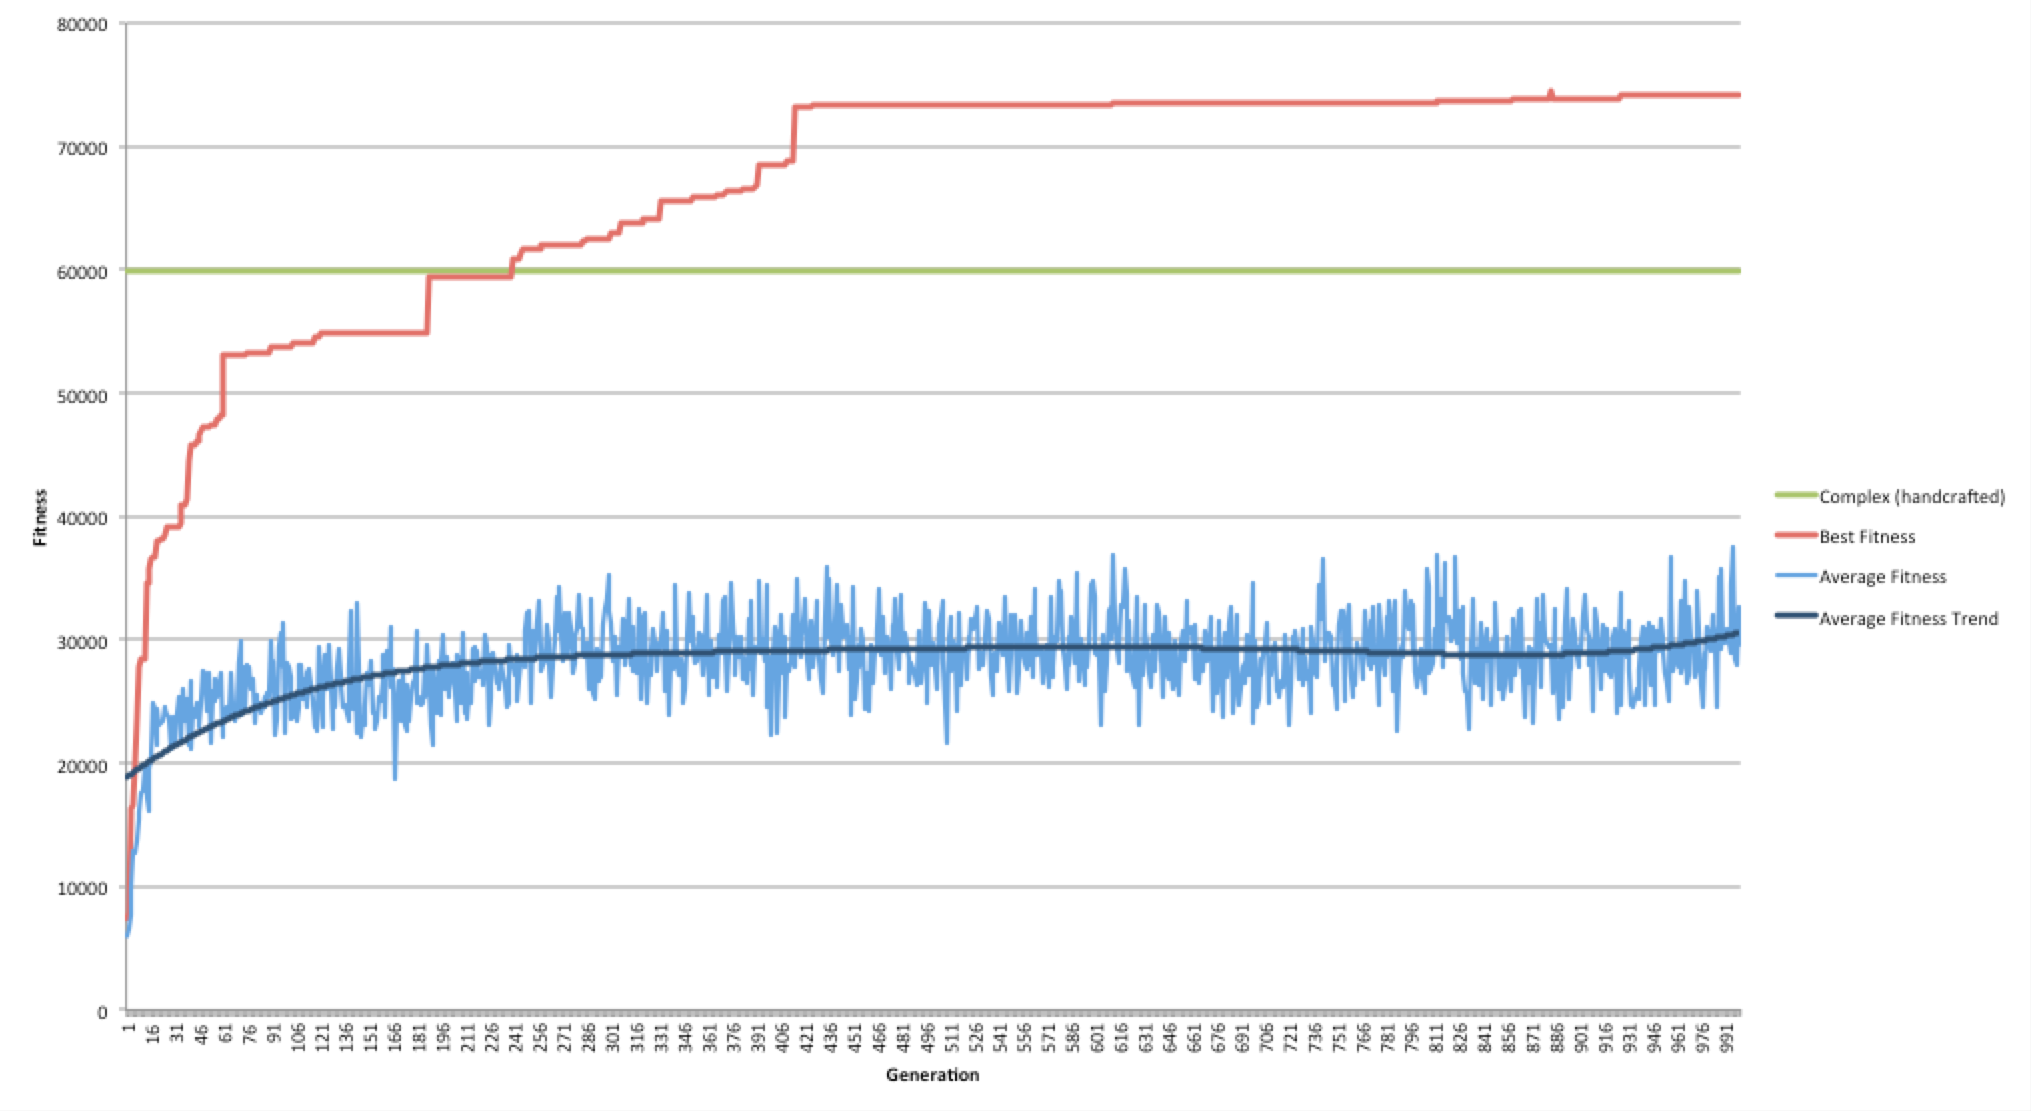
\includegraphics[scale=0.35]{FixSeedGraph.png}
	\caption{A learning run which had a fixed level seed of 323548323.}
	\label{fig:fixgraph}
\end{figure}

\begin{itemize}
\item It is evident from the graph that there is a lot of variance in both the best and average fitness between generations.
\item (Will include measurements of variance)
\item This could be explained by the rule based agent framework being sensitive to mutation, or the level playing module level seed affecting difficulty (explained further in Section \ref{sec:eval})
\item Due to this variance a learning run was performed that had a fixed level seed, so that each generation plays exactly the same levels, the graph is included as Figure \ref{fig:fixgraph}.
\item As expected (and due to the nature of $(\mu  + \lambda)$ ES) this removes all variance in the best fitness, but some still remains in average fitness.
\item Also the maximum fitness achieved by an agent in the run was higher.
\item (Graph also shows an issue with benchmark; non-determinism. The fitness jumps and falls at generation 882, this fitness calculation for the best agent was different between gen 882 and gen 883, and is unrepeatable in manual tests.)
\item The final agent produced from the fix seed run is included in the agent analysis below.
\end{itemize}

\subsubsection{Population Variance}

\begin{itemize}
\item Both graphs show a large difference between the best and average fitness. This suggest a large variance in fitness over a single population.
\item The last generation of the fix seed run has a standard deviation ...
\item As the ES ensures each generation's population are mutated from the previous best agents, this shows that the agent framework is particularly sensitive to mutation, which ruleset fitness dropping dramatically in one mutation round.
\end{itemize}

\clearpage
%-----------------------------------------------------------------------
% Learnt Agents
%-----------------------------------------------------------------------

\subsection{Learnt Agents}
\label{subsec:evallearnt}

\begin{itemize}
\item Three learnt agents were taken from the learning runs to be analysed here: the Learnt Difference agent, which performed best compared to the average fitness (past generation 800); the Learnt Best agent, which got the highest fitness overall (past generation 800) and the Learnt Fixed Seed agent, which was the final agent from the fixed seed run.
\item This section will compare them with the handcrafted agents, in both the learning evaluation task and the comparator task (Section \ref{subsec:comptask}).
\end{itemize}

\subsubsection{Learning Evaluation Task}

\begin{table}
  \begin{adjustwidth}{-0cm}{-0cm}
  \begin{center} \small
    \begin{tabular}{ | l | c | c | c | c |}
    \hline
    \textbf{Agent} & \textbf{Average} & \textbf{Offset} & \textbf{Best} & \textbf{Worst} \TBstrut \\ \thickhline
    \textbf{Complex} & 59,206 & 0 & 74,286 & 38,494  \\ \hline
    \textbf{Simple Reactive} & 37,310 & 21,896 & 61,784 & 19,526 \\ \hline
    \textbf{Forward Jumping} & 20,458 & 38,748 & 45,022 & 8,378 \\ \thickhline
    \textbf{Learnt Best} & 59,079 & 127 & 73,058 & 43,740  \\ \hline
    \textbf{Learnt Difference} & 58,930 & 276 & 72,672 & 36,440  \\ \hline
    \textbf{Learnt Fixed Seed} & 54,115 & 5,091 & 74,194 & 38,494  \\ \hline
    \end{tabular}
  \end{center}
  \end{adjustwidth}
  \caption{\small Statistics from handcrafted and learnt agents playing all the evaluation tasks from the final learning run.}
  \label{tab:learnrunagents}
\end{table}

\begin{itemize}
\item Three chosen learnt agents and three handcrafted agents were run through the each generation's evaluation task of the final learning task (i.e. 1000 tasks, with the same options, different seeds). Results are compiled in to Table \ref{tab:learnrunagents}
\item We can see from the data that both the Leant best and Learnt difference agents performed at the same level as the complex agent and considerable better than the other handcrafted agents. Which implies they became very capable at the task they were learning on.
\item We can also see that the learnt fixed seed agent did not perform quite as well, suggesting it became too suited to the single set of levels it was evolved over.
\item The large difference between best and worst fitness for each agent reiterates the problem of variance may stem from the level playing modules use of level seed, which may be overly affecting difficulty.
\end{itemize}

\clearpage
\subsubsection{Comparator Task}

\begin{table}
  \begin{adjustwidth}{-0cm}{-0cm}
  \begin{center} \small
    \begin{tabular}{ | l | c | c | c | c | c |}
    \hline
    & \textbf{Total} & \textbf{Levels} & \textbf{Enemies} & \Tstrut \\
    \textbf{Agent} & \textbf{Score} & \textbf{Completed} & \textbf{Killed} & \textbf{Distance} \Bstrut \\ \thickhline
    \textbf{Complex} & 1,758,931 & 168 (33\%) & 1,440 (8\%) & 62,231 (45\%) \\ \hline
    \textbf{Simple Reactive} & 1,102,733 & 87 (17\%) & 588 (3\%) & 44,038 (32\%) \\ \hline
    \textbf{Forward Jumping} & 954,141 & 65 (13\%) & 743 (4\%) & 38,484 (28\%) \\ \thickhline
    \textbf{Learnt Difference} & 1,521,200 & 144 (28\%) & 1,130 (6\%) & 55,710 (40\%) \\ \hline
    \textbf{Learnt Best} & 1,510,697 & 133 (26\%) & 1,603 (8\%) & 54,341 (39\%) \\ \hline
    \textbf{Learnt Fixed Seed} & 1,267,914 & 102 (20\%) & 1,173 (6\%) & 48,131 (35\%) \\ \hline
    \end{tabular}
  \end{center}
  \end{adjustwidth}
  \caption{\small Competitive statistics from handcrafted and learnt agents playing the comparator task with a seed of 1000.}
  \label{tab:learnagentcomp}
\end{table}

\afterpage{
\begin{landscape}
 \begin{figure}
  \centering
  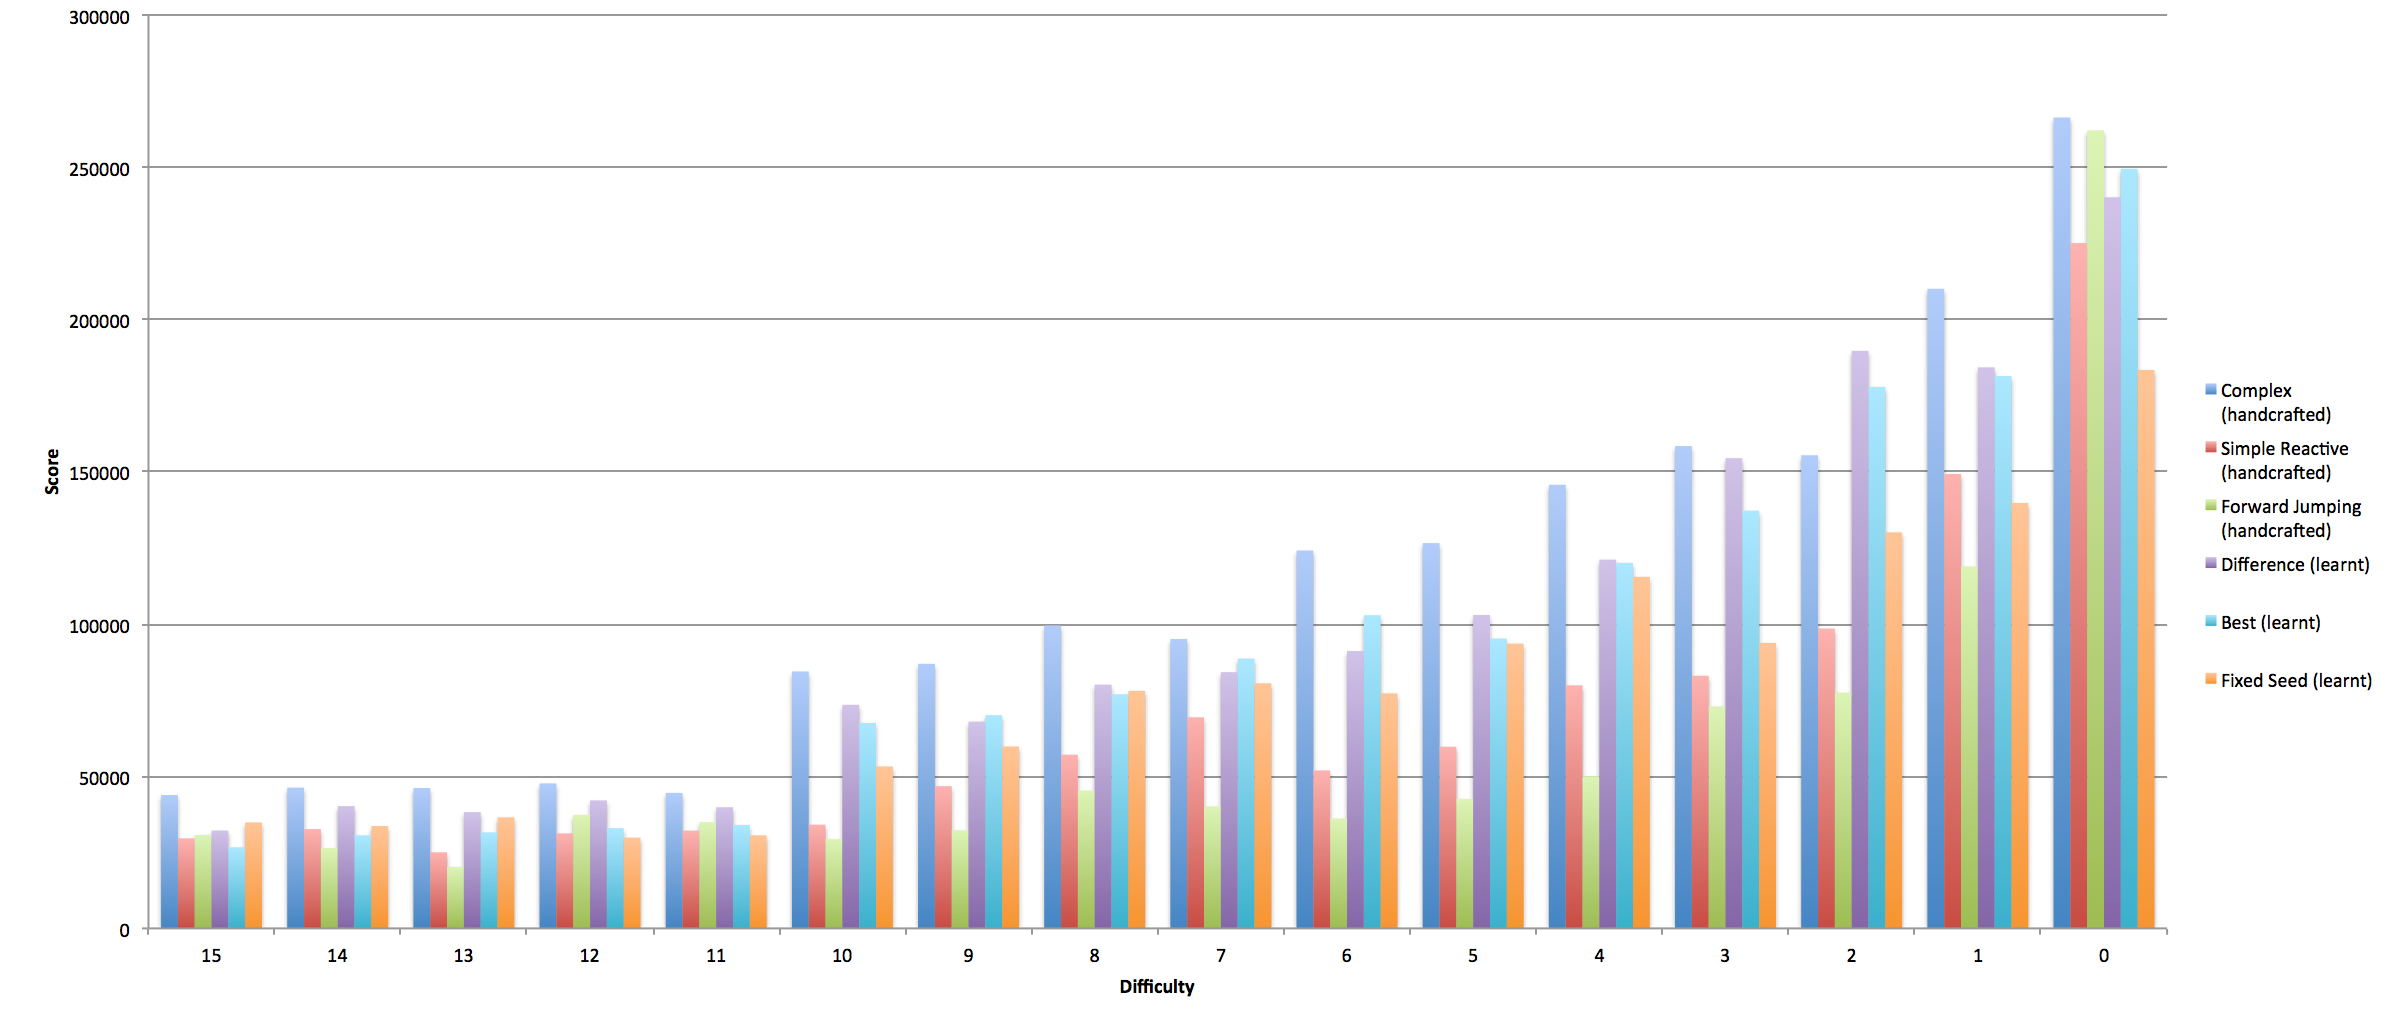
\includegraphics[scale=0.6]{CompTaskGraph.png}
  \caption{Graph charting the score achieved on different difficulty levels during the comparator task.}
  \label{fig:compgraph}
 \end{figure}
\end{landscape}
}

\begin{itemize}
\item Three chosen learnt agents and three handcrafted agents were run through the comparator task with seed of 1000. Results are compiled in to Table \ref{tab:learnagentcomp}
\item We can see from the data that both the Leant best and Learnt difference agents performed better than the two simpler handcrafted agents, but not as well as the complex agent. Considering the evaluation task result, this shows that the learning evaluation task it doesn't represent the comparator task well enough
\item We can also see that the learnt fixed seed agent did not perform quite as well, suggesting learning from many sets of levels helps when tackling different challenges.
\item Figure \ref{fig:compgraph} shows how the agents performed at different difficulties in the comparator task. Learnt agents were outperformed by complex agent on all difficulties (especially 6, 5 and 4) except 2, which was the most prevalent in the learning evaluation task. Implying that a longer and more representative task may produce a better agent.
\end{itemize}


%-----------------------------------------------------------------------
% Learnt Agent Behaviours
%-----------------------------------------------------------------------
\subsection{Learnt Agent Behaviours}

\begin{table}[t]
  \begin{adjustwidth}{-2cm}{-2cm}
  \begin{center} \scriptsize
    \begin{tabular}{ | c | c | c | c | c | c | c | c | c | c | c | c || c | c | c | c |}
    \hline
    \multirow{2}{*}{\textbf{\#}} & \multicolumn{11}{c ||}{\textbf{Conditions}} & \multicolumn{4}{c |}{\textbf{Actions}} \Tstrut \\ \cline{2-16}
    
	& \tiny MM & \tiny JA & \tiny OG & \tiny EL & \tiny EUR & \tiny ELR & \tiny OA & \tiny PA & \tiny PB & \tiny MX & \tiny MY & \tiny Left~ & \tiny Right & \tiny Jump~ & \tiny Speed \TBstrut \\ \thickhline
	1 & & & & & & & & & 1 & & 		& & T & T & T \\ \hline
	2 & & 1 & 1 & & & & 1 & 2 & 0 & & 		& & T & T & \\ \hline
	3 & & 0 & 0 & & & & 1 & 2 & 0 & & 		& & T & & \\ \hline
	4 & & 1 & 1 & & & & 0 & 2 & 0 & & 		& & T & & T \\ \hline
	5 & & 1 & 1 & & & & 0 & 1 & 0 & 2 & 		& & T & T & T \\ \hline
	6 & & 0 & 1 & & & & & 1 & 0 & 2 & 		& & T & & T \\ \hline
	7 & & 0 & 0 & & & & & 2 & 0 & 2 & 		& T & & & \\ \hline
	8 & & 0 & 0 & & & & & 1 & 0 & 2 & 1 		& T & & & T \\ \hline
	9 & & 0 & 0 & & & & & 1 & 0 & & 		& & T & T & T \\ \hline
	10 & & & 0 & & & 1 & & 0 & 0 & 2 & 1 		& T & & & T \\ \hline
	11 & & 0 & 1 & & & 1 & & 0 & 0 & & 		& & T & & \\ \hline
	12 & & & & & & 1 & & 0 & 0 & & 		& & T & T & \\ \hline
	13 & & & 0 & & & 1 & & 0 & 0 & & 		& & T & T & T \\ \hline
	14 & & & & & 1 & & 1 & 0 & 0 & & 		& T & & T & \\ \hline
	15 & & 0 & 1 & & & & 1 & 0 & 0 & & 		& & T & & \\ \hline
	16 & & & & & & & 1 & 0 & 0 & & 		& & T & T & T \\ \hline
	17 & & & & & & & 1 & 0 & 0 & 2 & 		& & T & T & \\ \hline
	18 & & & 1 & & & & & & & & 		& & T & & T \\ \hline
	
	-  & & & & & & & & & & & 		& & T & & \\ \hline
    \end{tabular}
  \end{center}
  \end{adjustwidth}
  \caption{Ruleset for learnt difference agent. Blank entries denote {\scriptsize DONT\_CARE} for Conditions and \textbf{false} for Actions.}
  \label{tab:LDA}
\end{table}

\begin{itemize}
\item Of the learnt agents the learnt difference agent performs the best in the comparator task
\item It also displays the most interesting behaviour which will be discussed here
\item A full ruleset for this agent is included in Figure \ref{} 
\end{itemize}






